\documentclass[letterpaper,12pt]{article}
\usepackage{tabularx} % extra features for tabular environment
\usepackage{tikz}
\usetikzlibrary{matrix,calc}
\usepackage{caption}
\usepackage{subfigure}
\usepackage{amsmath}  % improve math presentation
\usepackage{graphicx} % takes care of graphic including machinery
\usepackage[margin=1in,letterpaper]{geometry} % decreases margins
\usepackage{cite} % takes care of citations
\usepackage[final]{hyperref} % adds hyper links inside the generated pdf file
\hypersetup{
	colorlinks=true,       % false: boxed links; true: colored links
	linkcolor=blue,        % color of internal links
	citecolor=blue,        % color of links to bibliography
	filecolor=magenta,     % color of file links
	urlcolor=blue         
}
\usepackage{blindtext}
%++++++++++++++++++++++++++++++++++++++++


\begin{document}

\title{Assignment 1 Light Field Renderer}
\author{fanghzh1@shanghaitech.edu.cn}
\date{\today}
\maketitle


\tableofcontents
\section{Introduction}
The basic light field rendering is simply realized. By adjusting the xy coordinates of the virtual camera in the st plane and the z coordinates perpendicular to the st and uv planes, the perspective images at different positions are obtained. The simulation of the aperture is added, and the gradual change of the aperture is smoothed.
\section{Implement}
\subsection{Data Representation}
\begin{itemize}
\item[1]Input image like follow:
\begin{equation*}
P = 
\left.
\overbrace{
	\begin{bmatrix}
	C_{11} & . & . \\
	. & . & . \\
	. & . & C_{ij}
	\end{bmatrix}
}^{320}\right \}{240},C_{ij} = (R,G,B)
\end{equation*}
\item[2]We have 256 image for the data set,for computation locality,transform the data set:
\begin{equation*}
\begin{aligned}
matrix-2-image(P) = \overbrace{
	\begin{bmatrix}
	R_{1} & . & . & . & .& R_{k} \\
	G_{1} & . & . & . & .& G_{k} \\
	B_{1} & . & . & . & .& B_{k} \\
	\end{bmatrix}
}^{320*240}
\end{aligned}
\end{equation*}

\begin{equation*}
Data = 
\begin{bmatrix}
image-2-matrix(P)_{1}\\
. \\
. \\
. \\
transoform2matrix(P)_{256}\\
\end{bmatrix}
D\ is\ a\ ((256\ \times 3),(320 \times 240))matrix.
\end{equation*}
\item[3] We define two functions as using before:
\paragraph{Matrix 2 image and image 2 matrx}
Just reshape the matrix
\paragraph{Blend by weight}
Input photos like as $(wh,3)*n$,and the weight,Output $photos*weight$ as one image.
\end{itemize}
\subsection{GUI Design}
\begin{figure}[h]
	\centering 
	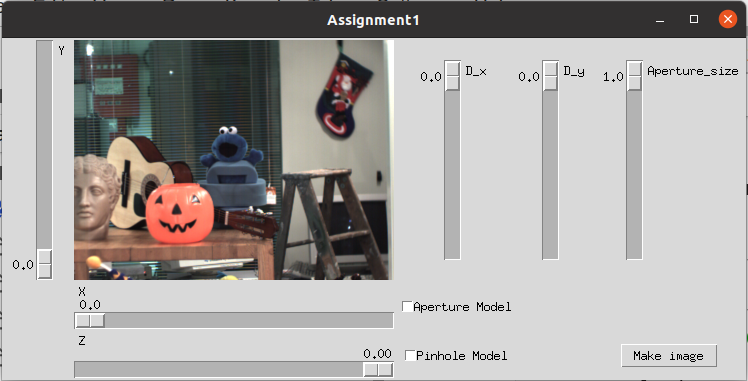
\includegraphics[width=0.7\textwidth]{Image/Gui.png}
	\caption{GUI}
\end{figure}
\begin{itemize}
	\item[1] 6 scale bars,the three around the image are used to adjust the xyz coordinates of the virtual camera, and the remaining three vertical scale bars are used to adjust the disparity in the x and y directions, and adjust the size of the aperture in the aperture mode.
	\item[2] 
	The adjustment range of xy is from 0 to 16, the adjustment range of z is from 0 to 1, where the zero point of (x, y) is set at the lower left corner of the st plane, and the 0 of z is set on the st plane.
	\item[3]
	The adjustment range of disparity is from -10 to 10, and the aperture size is from 1 to 10.
	\item[4]
	2 clickbox, choose if get the pinhole camera model or add add an aperture.
\end{itemize}

\subsection{Render System}
\subsubsection{Moving X and Y}
For we need getting the color blending by the nearest color,we should do the interpolation.Basic method blending from the 4 color,which have the form:
\begin{equation*}
\begin{aligned}
Camera(x,y)= \begin{bmatrix}
Color_1 & Color_2 & Color_3 & Color_4
\end{bmatrix}
\begin{bmatrix}
\omega_1 \\
\omega_2 \\
\omega_3 \\
\omega_4 \\
\end{bmatrix}
\end{aligned}
\end{equation*}
Where the $Color_1$ have the coordinate $(x_1,y_1)$,in the upper left corner of the square which include $(x,y)$: 
\begin{equation*}
\begin{aligned}
d_1 = x-x_1,\ d_2=y_1-y\\
\begin{bmatrix}
\omega_1 \\
\omega_2 \\
\omega_3 \\
\omega_4 \\
\end{bmatrix}
=
Normlization (
\begin{bmatrix}
(1-d_1)(1-d_2)\\
d_1 (1-d_2) \\
(1-d_1)d_2\\\
d_1 d_2 \\
\end{bmatrix}
)
\end{aligned}
\end{equation*}
Basic interpolating as follow:
\begin{figure}[h]
	\centering 
	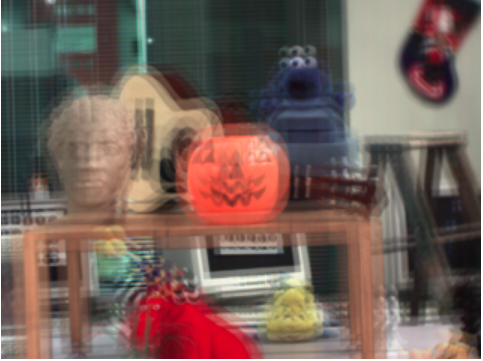
\includegraphics[width=0.5\textwidth]{Image/base.png}
	\caption{4 points interpolation without fix}
\end{figure}
\newpage
\subsubsection{Disparity}
The essence of Disparity is to adjust the view depth, enter the coordinates of the center position, and calculate the bias according to the surrounding coordinates.
\\
To calculate the disparity corrected image, we simply define it as three steps:
\paragraph{Disparity matrix}
Calculate the required offset according to the center coordinates and the disparity in the xy direction
\paragraph{Re image}Reconstruct a new picture based on the offset
\paragraph{Q interpolator2}Interpolate according to the new picture to obtain the required image
\begin{figure}[htbp]
	\centering
	\begin{minipage}[t]{0.48\textwidth}
		\centering
		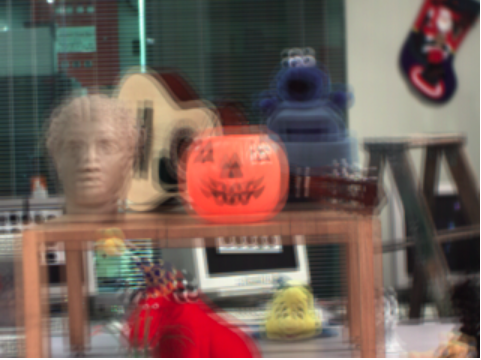
\includegraphics[width=6cm]{Image/-2.png}
		\caption{disparity(-2,2)}
	\end{minipage}
	\begin{minipage}[t]{0.48\textwidth}
		\centering
		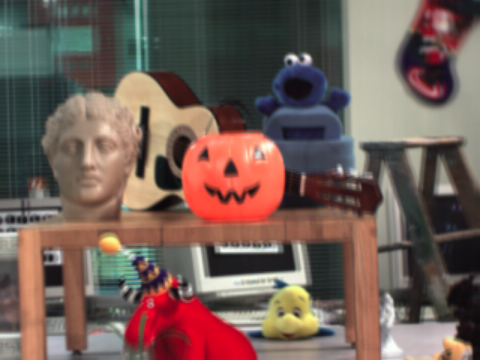
\includegraphics[width=6cm]{Image/dis.png}
		\caption{disparity(-8.3,5.6)}
	\end{minipage}
\end{figure}
\subsubsection{Moving Z}
When the z coordinate of the virtual camera is adjusted to move away from the uv plane, the required part of the light data does not exist and the image cannot be obtained. 
\\
Therefore, it can only move to a plane close to the uv, which is similar to the image that has been obtained, keeping the center position unchanged, first performing proportional cropping, and then zooming in.Define as function scale by z.

\begin{figure}[htbp]
	\centering
	\begin{minipage}[t]{0.48\textwidth}
		\centering
		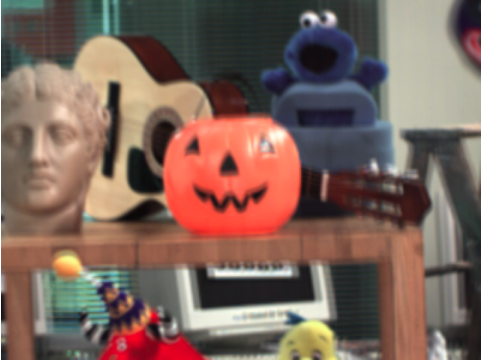
\includegraphics[width=6cm]{Image/0.75.png}
		\caption{Z = 0.75}
	\end{minipage}
	\begin{minipage}[t]{0.48\textwidth}
		\centering
		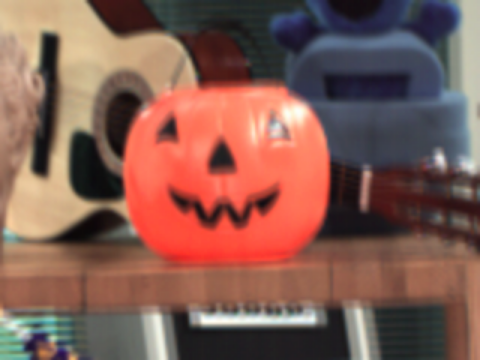
\includegraphics[width=6cm]{Image/0.5.png}
		\caption{Z = 0.5}
	\end{minipage}
\end{figure}

\subsubsection{Aperture}
\paragraph{Aperture model}
\begin{itemize}
	\item[1]Think of the aperture as a circle with the input coordinates as the center and radius d, and this circle falls on the st plane.
	\item[2]The st plane has been gridded, and each point has a real camera image. The virtual image formed by the aperture should be synthesized using the points in the circle.
	\item[3]In order to make the image generated by the iris gradual, it is necessary to consider not only the points inside the circle, but also the nearest point outside the circle
\end{itemize}
\paragraph{Model the weight}
Discuss the weight of each image participating in the synthesis:
\begin{itemize}
	\item[1]For $point_i \in all\ points\ arround$ Calculate the Euclidean distance to the center coordinates $d_i \in D\ for\ point_i$
	\item[2]For the points inside the circle, the weight of the distance part is fully included as 1. For the points outside the circle, use $r/d$ to linearly weaken the weight, and gradually increase with r until the complete weight is obtained 1.
	\item[3]Regularization, so that the sum of weights is 1.
	\item[4]Gaussian filtering\\
	We want to keep mainly the light close to the coordinate center, so we use Gaussian probability density function to process again.
\end{itemize}
\paragraph{Generate image with aperture}
First give a complete aperture calculation method
\begin{itemize}
	\item[1]Input the center, also use$(8.4,8.6)$.Consider that the size of the aperture is 2, and then find the closest layer of points inside the aperture and outside the aperture, as shown in the figure, the green point is the center position, the red is the first layer outside the circle, and the blue is the inside of the circle points.Because all weights are not taken outside the circle. For smooth, the actual weights after mapping are green points
	\begin{figure}[h]
		\centering 
		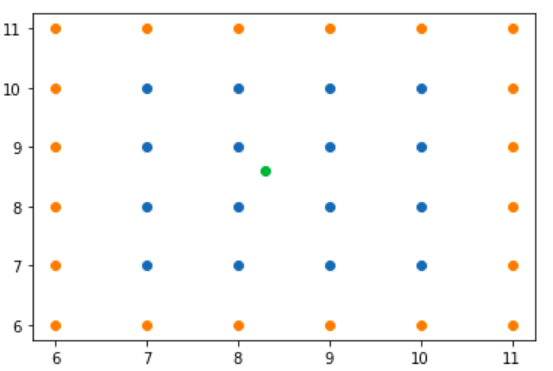
\includegraphics[width=0.5\textwidth]{Image/center.png}
		\caption{Points involved}
	\end{figure}
	\item[2]According to the method mentioned above, the weights are calculated and mapped to the Gaussian distribution $ scale = aperture\ size =2$,Blue is the inner circle points, orange is the outer circle.
	\begin{figure}[h]
	\centering 
	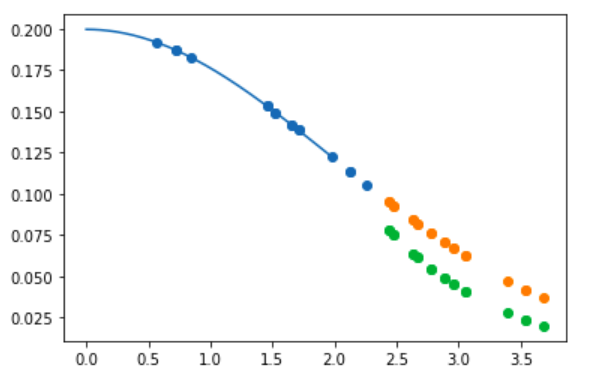
\includegraphics[width=0.5\textwidth]{Image/weight.png}
	\caption{Gaussian mapping}
	\end{figure}

	\item[3]
	In order to better reflect the focus of the weight, make the following visualization, you can see that the closer to the center of the coordinate, the greater the weight obtained.
	\begin{figure}[h]
	\centering 
	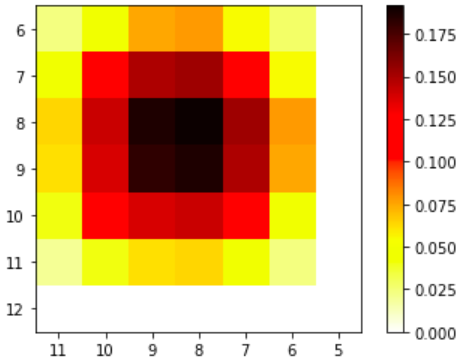
\includegraphics[width=0.5\textwidth]{Image/heat.png}
	\caption{Weight focus}
	\end{figure}
	\newpage
	\item[4]The rest of the processing methods are similar, so I won’t repeat them.It can be seen that there is a more obvious blur in the background part, obtained are as follows.
	\begin{figure}[htbp]
		\centering
		\begin{minipage}[t]{0.48\textwidth}
			\centering
			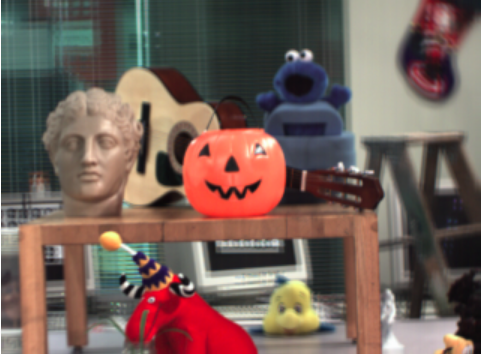
\includegraphics[width=6cm]{Image/size0.png}
			\caption{Pinhole}
		\end{minipage}
		\begin{minipage}[t]{0.48\textwidth}
			\centering
			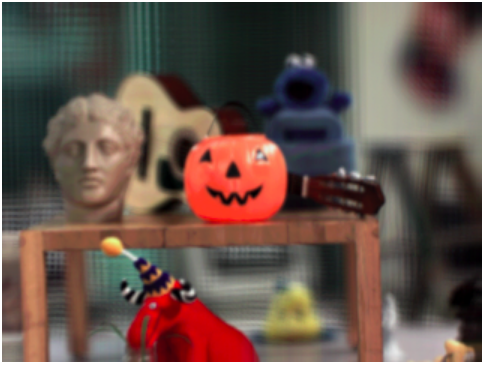
\includegraphics[width=6cm]{Image/size2.png}
			\caption{Aperture}
		\end{minipage}
	\end{figure}

\end{itemize}
\section{Experiments}
\subsection{What do you observe if you use interpolation on undersampled light field?}
\begin{itemize}
\item[1]If the image set is undersampled, this mean we have the less information to interpolation,which would case more ghosting. 
\item[2]As an experiment,let's cut the image set from$16 \times 16$ into $8 \times 8$ in the same view range,than sample the $(9,9)$ and $(4.5,4.5)$,which mean the same direction.
\begin{figure}[htbp]
	\centering
	\begin{minipage}[t]{0.48\textwidth}
		\centering
		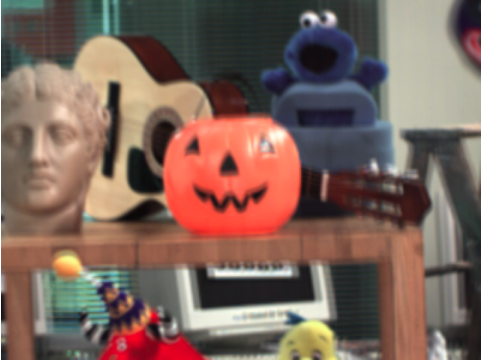
\includegraphics[width=6cm]{Image/0.75.png}
		\caption{From 16 $\times$ 16}
	\end{minipage}
	\begin{minipage}[t]{0.48\textwidth}
		\centering
		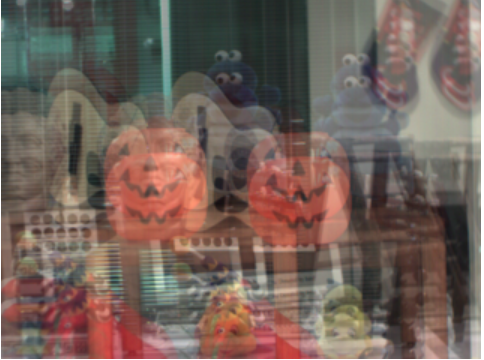
\includegraphics[width=6cm]{Image/64.png}
		\caption{From 8 $\times$ 8}
	\end{minipage}
\end{figure}
\end{itemize}
\subsection{What happens when you move your focal plane from far to near?}
\begin{itemize}
	\item[1]Move the focal plane from far to near, is equal to adjust disparity. Showig as this two sampled from $[8.4,8.6]$
		\begin{figure}[h]
		\centering
		\begin{minipage}[t]{0.48\textwidth}
			\centering
			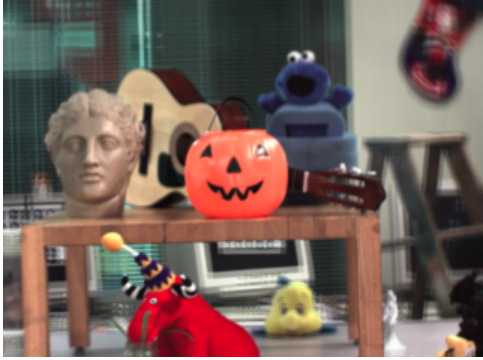
\includegraphics[width=6cm]{Image/FF.png}
			\caption{Near}
		\end{minipage}
		\begin{minipage}[t]{0.48\textwidth}
			\centering
			\includegraphics[width=6cm]{Image/Far.png}
			\caption{Far}
		\end{minipage}
	\end{figure}
	\item[2]From the basic image,move the focal to the near place, like showing in $2.3.2$.The pumpkin and red doll in the front position become clearer, and the object and chair in the upper right corner become more blurred.
	\item[3]As for move to far,the scenery in the distance becomes clear. You can mainly see the ornaments in the upper right corner and the ladder on the right, but compared to the previous picture, the pumpkin becomes more blurred.
\end{itemize}
\subsection{Which focal plane gives you the optimal results (least aliased reconstruction)?}
It depends on the object you want to focus on. Such as Figure Pinhole is a well result in my opinion.
\subsection{What happens when you increase the size of the aperture?}
\subsubsection{Weight change}
Let's increase the size of the aperture to 4, at this time each pixel participates in the synthesis of 100 rays.At this time, the effect of weight mapping is as follows.The more scattered the samples are, the mutual bias will be equalized, and the position far away from the aperture will be blurred.
	\begin{figure}[htbp]
	\centering
	\begin{minipage}[t]{0.48\textwidth}
		\centering
		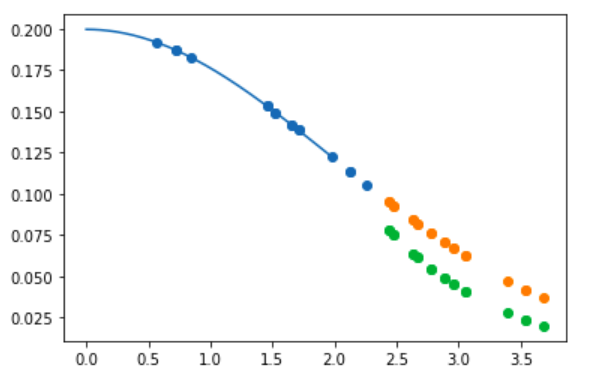
\includegraphics[width=6cm]{Image/weight.png}
		\caption{size=2}
	\end{minipage}
	\begin{minipage}[t]{0.48\textwidth}
		\centering
		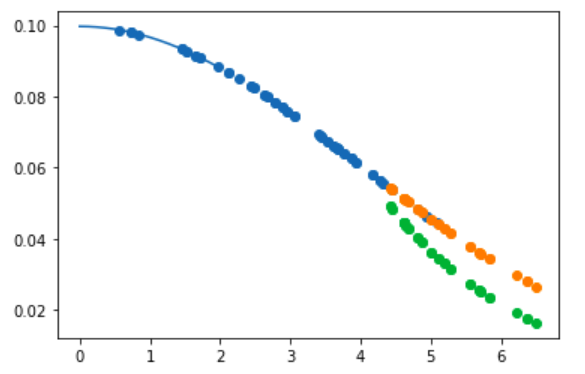
\includegraphics[width=6cm]{Image/size4w.png}
		\caption{size=4}
	\end{minipage}
\end{figure}
\subsubsection{View}
The blurring of the background is more obvious and darker.
	\begin{figure}[htbp]
	\centering
	\begin{minipage}[t]{0.48\textwidth}
		\centering
		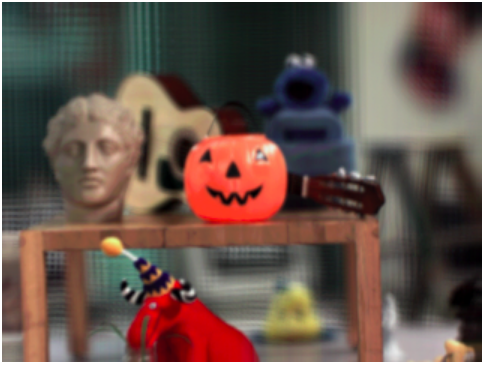
\includegraphics[width=6cm]{Image/size2.png}
		\caption{size=2}
	\end{minipage}
	\begin{minipage}[t]{0.48\textwidth}
		\centering
		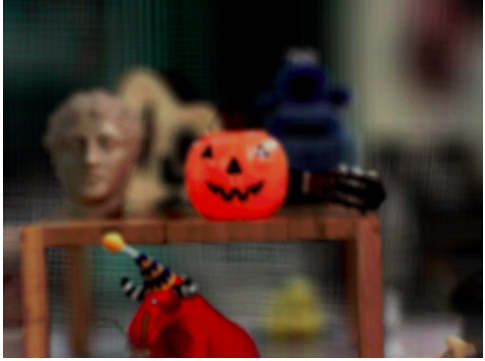
\includegraphics[width=6cm]{Image/size4.png}
		\caption{size=4}
	\end{minipage}
\end{figure}

\section{Supplement}
\subsection{Implement the z directional motion of the camera}
See scale by Z
\begin{equation*}
\begin{aligned}
\frac{d}{D} = Z^{'},Photo\ size = (W,H)\\
New\ image = Photo[W(\frac{1}{2}-\frac{d}{2D}):W(\frac{1}{2}+\frac{d}{2D}),H(\frac{1}{2}-\frac{d}{2D}):H(\frac{1}{2}+\frac{d}{2D})]
\end{aligned}
\end{equation*}

\subsection{Making the view smoothly changed when increase the size of the aperture}
See "Model the weight" part.Mainly add the nearest circle outside the circle, and then add the distance weight.
\section{Conclusion}
\subsection{algorithms}
\paragraph{Brightness after blending}
Because of the weighting and then regularization in the synthesis,physically, the larger the aperture, the brighter the scene, but the resulting composite will be darker,but directly add a plus would make overflow.
	\begin{figure}[htbp]
	\centering
	\begin{minipage}[t]{0.48\textwidth}
		\centering
		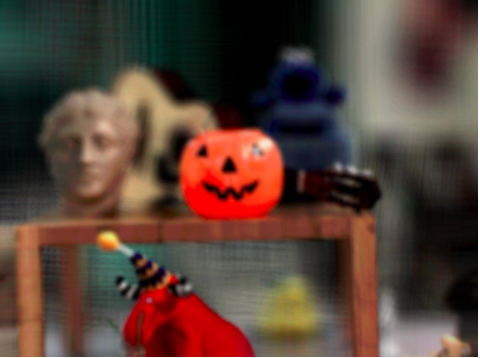
\includegraphics[width=6cm]{Image/size4l.png}
		\caption{Lighter}
	\end{minipage}
	\begin{minipage}[t]{0.48\textwidth}
		\centering
		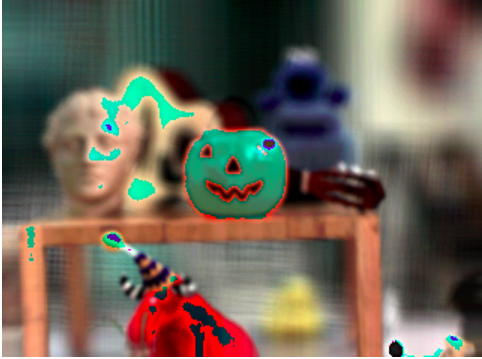
\includegraphics[width=6cm]{Image/size4o.png}
		\caption{Overflow}
	\end{minipage}
\end{figure}

Currently this parameter can only be adjusted manually.
\paragraph{Gaussian filtering parameters}
The scale of the Gaussian distribution affects the weight.According to the previous conclusions, the larger the scale, the smoother it will cause the darker the background
\begin{figure}[h]
	\centering 
	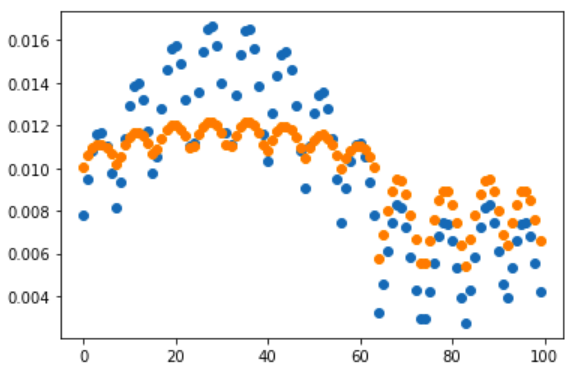
\includegraphics[width=0.5\textwidth]{Image/smooth.png}
	\caption{scale = 0.5size and size}
if we add to 3size
\end{figure}
\newline
If we add to 3size,The brightness is very low, but the blur is also obvious
	\begin{figure}[htbp]
	\centering
	\begin{minipage}[t]{0.48\textwidth}
		\centering
		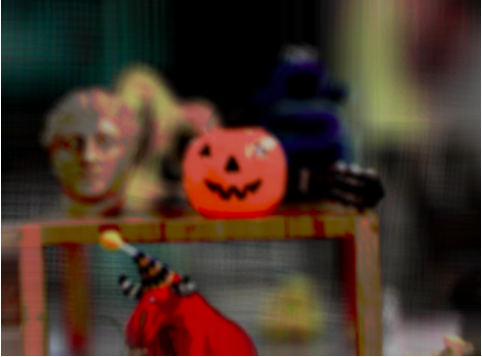
\includegraphics[width=6cm]{Image/3g.png}
		\caption{scale=3 $\times$size}
	\end{minipage}
	\begin{minipage}[t]{0.48\textwidth}
		\centering
		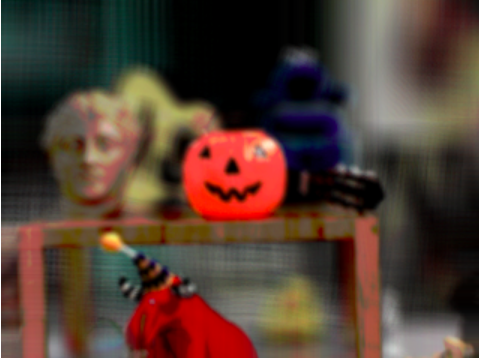
\includegraphics[width=6cm]{Image/3gl.png}
		\caption{Lighter}
	\end{minipage}
\end{figure}


\subsection{performance}
\paragraph{Fix disparity for lots of image}
Numpy is difficult to control locality,I promise to use C++ implementation next time.



\end{document}